\documentclass[a0,portrait]{a0poster}
\usepackage[most]{tcolorbox} % For drawing colored boxes
\usepackage{multicol} % This is used to split the poster into multiple columns
\usepackage{graphicx} % Allows including images
\usepackage{xcolor} % Allows for color changes
\usepackage{tabulary}
\usepackage{colortbl}
\usepackage{helvet} % Uses Helvetica font for a more modern look
\usepackage[utf8]{inputenc} % Encoding
\usepackage{amsmath, amsthm, amssymb, amsfonts} % Math packages
\usepackage{tikz} % For drawing shapes and effects
\usepackage{XCharter} % A modern and refined font choice
\usepackage{lipsum} % Generates filler text
\usepackage{commath}
\usepackage{hyperref}

\usepackage{geometry}
\geometry{a0paper,left=.5in,right=.5in,top=1in,bottom=1.5in,heightrounded}
% Set the background color to white
\pagecolor{white}

% Define a contemporary color palette
\definecolor{TitleColor}{RGB}{63, 81, 181} % Deep blue
\definecolor{SectionColor}{RGB}{255, 87, 34} % Vibrant orange
\definecolor{SubsectionColor}{RGB}{0, 150, 136} % Teal
\definecolor{TextColor}{RGB}{33, 33, 33} % Almost black
% Define a color palette
\definecolor{MainColor}{RGB}{0, 130, 202} % A deep blue color for key elements
\definecolor{AccentColor}{RGB}{255, 179, 0} % An accent color for highlights
\definecolor{BackgroundColor}{RGB}{255, 255, 255} % A white background for readability
%\definecolor{TextColor}{RGB}{0, 0, 0} % Black color for text for maximum contrast

% Font settings
\renewcommand{\familydefault}{\sfdefault}

% tcolorbox settings
\tcbset{
	colback=white, % Background color of the box
	colframe=SectionColor, % Color of the frame
	coltitle=TextColor, % Color of the title text
	fonttitle=\bfseries, % Bold title text
	left=6pt, % Space to the left inside the box
	right=6pt, % Space to the right inside the box
	boxsep=4pt, % Space between text and frame
	arc=2pt, % The arc of the box corners
	boxrule=1pt, % Thickness of the frame
	title style={left color=SectionColor!60!white, right color=SectionColor!60!white}, % Gradient on the title
	title filled % Fill the background of the title
}

% Customize the section boxes
\newtcolorbox{sectionbox}{
	colback=BackgroundColor,
	colframe=MainColor,
	coltitle=MainColor,
	fonttitle=\bfseries\large,
	boxrule=2pt,
	arc=10pt,
	boxsep=10pt,
	left=20pt,
	right=20pt,
	top=5pt,
	bottom=5pt,
	breakable,
	enhanced
}

\usepackage{graphicx}
\usepackage{tikz}
\usepackage{tikz-cd}
\usetikzlibrary{calc}
\usetikzlibrary{arrows, arrows.meta, positioning, shapes, shapes.multipart}
\usetikzlibrary{positioning,shapes.geometric}
\usepackage{pgfplots}
\pgfplotsset{compat=1.16}
\usepackage{caption}
\usepackage[absolute,overlay]{textpos}

%Listing
\usepackage{listings} %Code
\renewcommand{\lstlistingname}{Code}%

\definecolor{codegreen}{rgb}{0,0.6,0}
\definecolor{codegray}{rgb}{0.5,0.5,0.5}
\definecolor{codepurple}{rgb}{0.58,0,0.82}
\definecolor{backcolour}{rgb}{1,1,1}


\lstdefinestyle{sage}{
	language=Python,
	backgroundcolor=\color{white},
	basicstyle=\small\ttfamily\color{black}, 
	basicstyle=\footnotesize\ttfamily\color{black},
	keywordstyle=\color{blue!60!black},
	commentstyle=\color{green!60!black},
	stringstyle=\color{purple!60!black},
	showstringspaces=false,
	breaklines=true,
	tabsize=4,
	morekeywords={True, False, None},
	frame=leftline, % Remove the border
	framesep=3pt,
	frameround=tttt,
	framexleftmargin=3pt,
	numbers=left,
	numberstyle=\small\color{gray},
	xleftmargin=15pt, % Increase the left margin
	xrightmargin=5pt,
	captionpos=b,
	belowskip=0pt,
	aboveskip=4pt
}

\newcommand{\img}{\operatorname{\textnormal{Img}}}
\newcommand{\id}{\operatorname{\textnormal{Id}}}

\newcommand{\inv}[1]{#1^{-1}}

\newcommand{\ie}{\textnormal{i.e.}}
\newcommand{\eg}{\textnormal{e.g.}}

\newcommand{\of}[1]{\left( #1 \right)}

\newcommand{\sol}{\textcolor{magenta}{\bf Solution}}

\newcommand{\KeyGen}{\mathsf{KeyGen}}
\newcommand{\Enc}{\mathsf{Enc}}
\newcommand{\Dec}{\mathsf{Dec}}
\newcommand{\scheme}{\Sigma}
\newcommand{\keyspace}{\mathcal{K}}
\newcommand{\messagespace}{\mathcal{M}}
\newcommand{\ciphertextspace}{\mathcal{C}}

\newcommand{\library}{\mathcal{L}}
\newcommand{\zero}{\textcolor{red}{\texttt{0}}}
\newcommand{\one}{\textcolor{red}{\texttt{1}}}

\newcommand{\tab}{\hspace{12pt}}
\newcommand{\xor}{\oplus}
\newcommand{\adversary}{\mathcal{A}}
\newcommand{\isequal}{\overset{?}{=}}
\newcommand{\linking}{\diamond}

\newcommand{\true}{\texttt{true}}
\newcommand{\false}{\texttt{false}}
\newcommand{\randomness}{\$}
\newcommand{\uniform}{\xleftarrow{\randomness}}
\newcommand{\binaryfield}{\set{\zero,\one}}

\newcommand{\ctxt}{\texttt{CTXT}}
\newcommand{\eavesdrop}{\texttt{Eavesdrop}}

\newcommand{\otp}{\mathsf{OTP}}
\newcommand{\potp}{\mathsf{pOTP}}
\newcommand{\ots}{\mathsf{ots}}
\newcommand{\sL}{\mathsf{L}}
\newcommand{\sR}{\mathsf{R}}
\newcommand{\indexbit}{\texttt{Idx}}
\newcommand{\outbit}{\texttt{Out}}
\newcommand{\real}{\mathsf{real}}
\newcommand{\rand}{\mathsf{rand}}
\newcommand{\prf}{\mathsf{PRF}}

\newcommand*{\indist}{%
	\mathrel{\vcenter{\offinterlineskip
			\hbox{$\sim$}\vskip-.35ex\hbox{$\sim$}\vskip-.35ex\hbox{$\sim$}}}}

\newcommand{\outputs}{\Rightarrow}

% Begin the document
\begin{document}
	
	% Title section with a modern art feel
	\begin{minipage}[b]{1.0\linewidth}
		\centering
		\begin{textblock*}{1cm}(69cm,0cm) % {block width} (coords)
			
\includegraphics[scale=3.8]{school_logo.png}
		\end{textblock*}
		\veryHuge \color{TitleColor} \textbf{Pseudo-Random Generators and Functions} \\[0.5cm]
		\huge \textit{Unveiling the Complexity and Elegance of Randomness}\\[1cm]
		\LARGE\textcolor{SectionColor}{\textbf{Ji Yong-Hyeon \& Kim Dong-Hyeon}} \\[0.5cm]
		\large Department of Information Security, Cryptology, and Mathematics \\[0.25cm]
		\normalsize {\texttt{hacker3740@gmail.com, bob@university.cs}} \\
	\end{minipage}
	
	% Add some artistic shapes to the title using TikZ
	
\begin{tikzpicture}[overlay]
		\draw[TitleColor, line width=2cm] (-.5cm, -1) -- (81cm, -1); % Horizontal line with color
		\draw[TitleColor, line width=2cm] (-.5cm, -102) -- (81cm, -102); % Horizontal line with color
		\draw[SectionColor, line width=2cm, rotate=45] (15cm, -1cm) -- (15cm, 15cm); % Diagonal line with color
	\end{tikzpicture}
	
	\vspace{2.5cm} % Space after the title
	
	% Begin the body of the poster
	\begin{multicols}{2}
		
		% Introduction
		\begin{sectionbox}
			\section*{\textcolor{MainColor}{I.1 Introduction of PRG}}
			A deterministic function $G:\binaryfield^\lambda\to\binaryfield^{\lambda+l}$ with $l>0$ is a \textbf{secure pseudorandom generator (PRG)} if $\library_{\mathsf{PRG}-\mathsf{real}}^G\indist\library_{\mathsf{PRG}-\mathsf{rand}}^G$, where: \begin{center}
					\begin{tabular}{|c|}
						\hline
						\cellcolor{blue!25}$\library_{\mathsf{PRG}-\mathsf{real}}^G$\\
						\hline
						\begin{tabular}{l}
							\underline{\texttt{Query}():}\\
							\tab $s\gets\binaryfield^\lambda$\\
							\tab \textbf{return} $G(s)$
						\end{tabular}\\
						\hline
					\end{tabular}\quad\quad\quad
					\begin{tabular}{|c|}
						\hline
						\cellcolor{blue!25}$\library_{\mathsf{PRG}-\mathsf{rand}}^G$\\
						\hline
						\begin{tabular}{l}
							\underline{\texttt{Query}():}\\
							\tab $r\gets\binaryfield^{\lambda+l}$\\
							\tab \textbf{return} $r$
						\end{tabular}\\
						\hline
					\end{tabular}
			\end{center}
			\ \\
			We illustrate the distributions, for a length doubling ($l=\lambda$) PRG (not drawn to
			scale):
			\begin{center}
				\begin{minipage}{.45\textwidth}\centering
					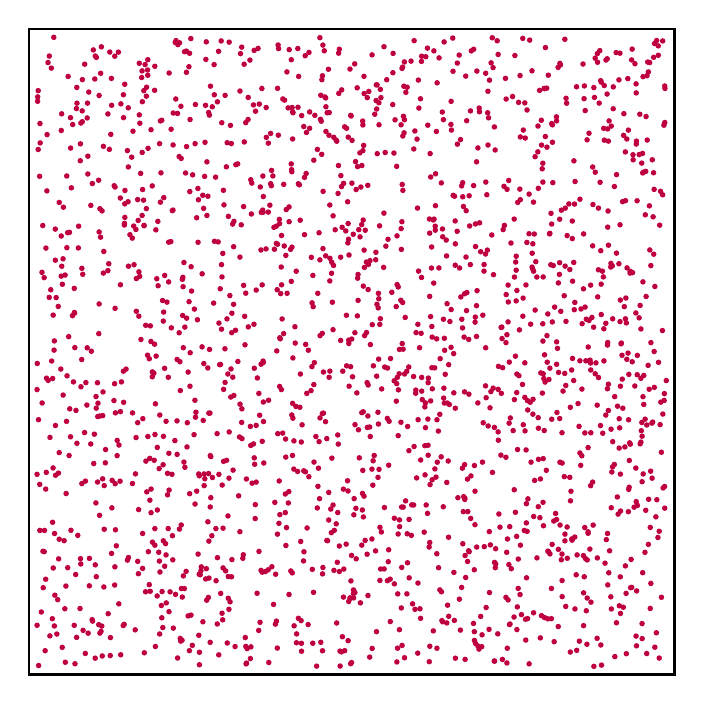
\begin{tikzpicture}
						% Pseudorandom distribution
						\foreach \i in {1,...,2000}{
							% Generate random points within the square
							\pgfmathsetmacro{\x}{rand*4}
							\pgfmathsetmacro{\y}{rand*4}
							\fill[purple] (\x,\y) circle (1pt);
						}
						\draw[thick] (-4.1,-4.1) rectangle (4.1,4.1) node[below left] {};
%						\node at (0, -2.5) {$\binaryfield^{\lambda}\to\binaryfield^{2\lambda}$};
					\end{tikzpicture}
					\captionof*{figure}{Pseudorandom dist. ($\binaryfield^\lambda\to\binaryfield^{2\lambda}$)}
				\end{minipage}
				\begin{minipage}{.45\textwidth}\centering
					
\begin{tikzpicture}% Uniform distribution
						\begin{scope}[shift={(5,0)}]
							%			\foreach \x in {-1.6,-1.5,...,1.6}{
								%				\foreach \y in {-1.6,-1.5,...,1.6}{
									%					\fill (\x,\y) circle (1pt);
									%				}
								%			}
							\fill[purple] (-4.1,-4.1) rectangle (4.1,4.1);
							\draw[thick] (-4.1,-4.1) rectangle (4.1,4.1) node[below left] {};
%							\node at (0, -2.5) {$\binaryfield^{2\lambda}$};
						\end{scope}
					\end{tikzpicture}
					\captionof*{figure}{Uniform dist. ($\binaryfield^{2\lambda}$)}
				\end{minipage}
			\end{center}
		\end{sectionbox}
		\begin{sectionbox}
			\section*{\textcolor{MainColor}{I.2 How \textcolor{red}{NOT} to Build a PRG}}
			A straightforward approach for the PRG might be to duplicate its input string.
			\begin{center}
				\begin{tabular}{|l|}
					\hline
					\underline{$G(s)$:}\\
					\tab return $s\parallel s$\\
					\hline
				\end{tabular}
			\end{center}
			For example, the following strings look likely they were sampled uniformly from $\binaryfield^8$:
			\[
			\one\one\zero\one\one\one\zero\one, \zero\one\one\one\zero\one\one\one,
			\zero\one\zero\zero\zero\one\zero\zero, \cdots
			\]
			\textbf{Comparison of Normalized Distributions:}
			\begin{center}
				\begin{minipage}{\textwidth}\centering
					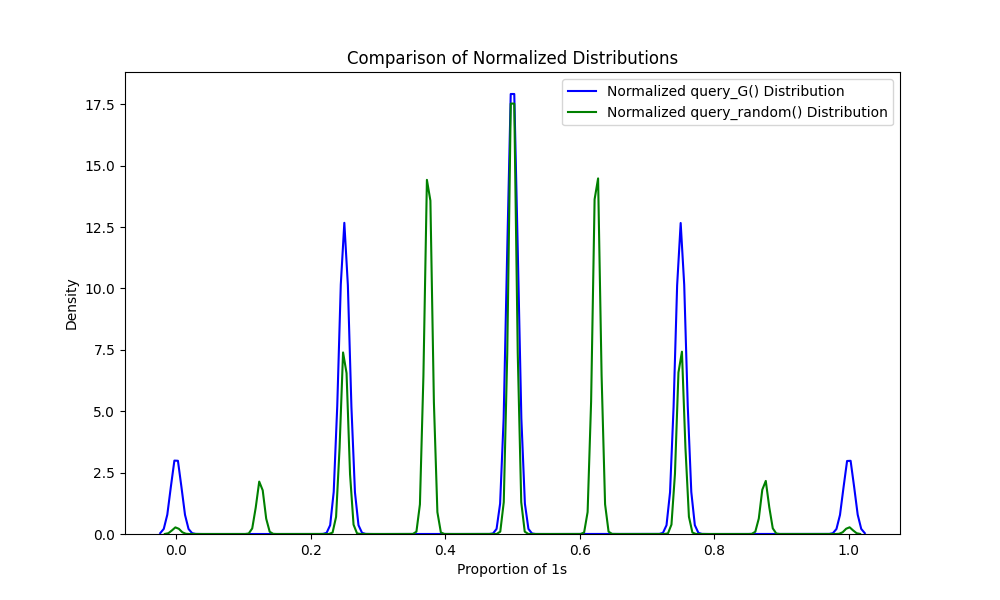
\includegraphics[scale=1]{query_8.png}
					\captionof*{figure}{$\lambda=4$, \ie, $\binaryfield^8$ with 1,000,000 experiments.}
				\end{minipage}
				\begin{minipage}{\textwidth}\centering
					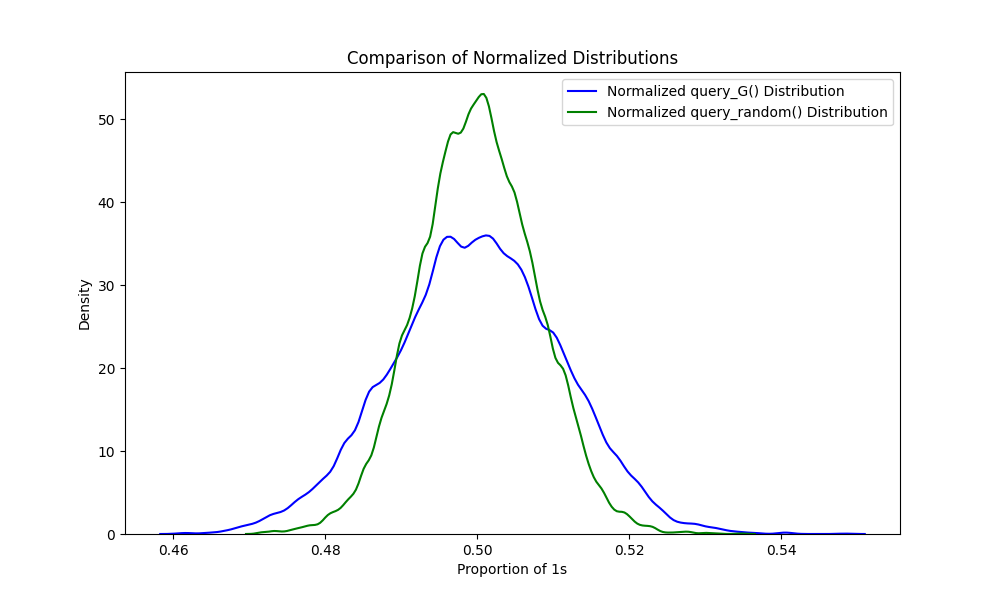
\includegraphics[scale=1]{query_1024.png}
					\captionof*{figure}{$\lambda=1024$, \ie, $\binaryfield^{2048}$ with 100,000 experiments}
				\end{minipage}
			\end{center}
\begin{lstlisting}[style=sage]
import numpy as np
import matplotlib.pyplot as plt
import seaborn as sns

def G(s):
	return s * 2
def query_G():
	lambda_length = 1024
	s = np.random.randint(0, 2, lambda_length).tolist()
	return G(s)

def query_random():
	lambda_length = 1024
	l_length = 1024
	r = np.random.randint(0, 2, lambda_length + l_length).tolist()
	return r

num_experiments = 100000
outputs_G = [query_G() for _ in range(num_experiments)]
outputs_random = [query_random() for _ in range(num_experiments)]
sums_G = [sum(output) for output in outputs_G]
sums_random = [sum(output) for output in outputs_random]
norm_sums_G = [s / 2048 for s in sums_G]
norm_sums_random = [s / 2048 for s in sums_random]
plt.figure(figsize=(10, 6))
sns.kdeplot(norm_sums_G, bw_adjust=0.5, label='Normalized query_G() Distribution', color='blue')
sns.kdeplot(norm_sums_random, bw_adjust=0.5, label='Normalized query_random() Distribution', color='green')

plt.legend()
plt.title('Comparison of Normalized Distributions')
plt.xlabel('Proportion of 1s')
plt.ylabel('Density')
plt.show()
\end{lstlisting}
		\end{sectionbox}
		
		\columnbreak
		\begin{sectionbox}
			\section*{\textcolor{MainColor}{II.1 Introduction of PRF}}
			This research explores groundbreaking concepts...
			\begin{center}
				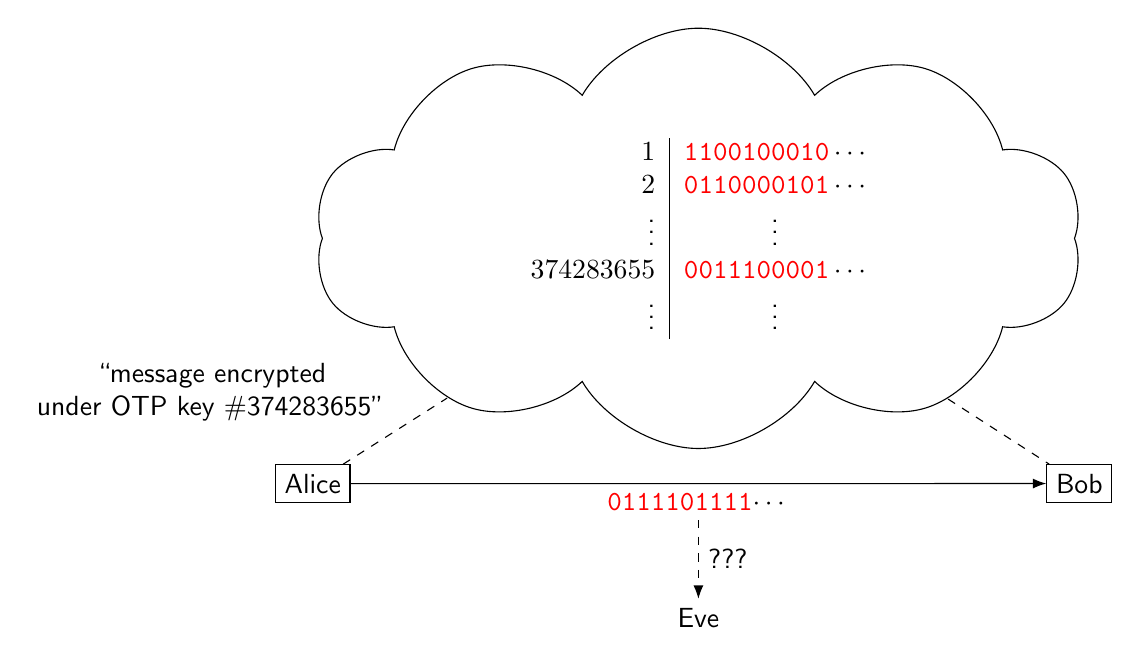
\begin{tikzpicture}[auto]
					% Cloud
					\node[cloud, draw, cloud puffs=10, cloud puff arc=120, aspect=2.5, inner ysep=.2em] (cloud) {
						$\begin{array}{r|c}
							1& \one\one\zero\zero\one\zero\zero\zero\one\zero\cdots\\
							2& \zero\one\one\zero\zero\zero\zero\one\zero\one\cdots\\
							\vdots&\vdots\\
							374283655& \zero\zero\one\one\one\zero\zero\zero\zero\one\cdots\\
							\vdots&\vdots
						\end{array}$
					};
					
					% Alice
					\node[draw, rectangle, below left=of cloud] (alice) {Alice};
					\draw[dashed] (alice) -- (cloud) node[midway, align=center] {``message encrypted\\under OTP key \#374283655''};
					
					% Bob
					\node[draw, rectangle, below right=of cloud] (bob) {Bob};
					\draw[dashed] (cloud) -- (bob);
					
					\draw[-Latex] (alice) -- (bob) node[midway,below] (ab) {\zero\one\one\one\one\zero\one\one\one\one$\cdots$};
					
					% Eve
					\node[below=1cm of ab] (eve) {Eve}; 
					\draw[dashed, -Latex] (ab) -- (eve) node[midway, align=center, right] {???};
				\end{tikzpicture}
			\end{center}
			The goal of a pseudorandom function is to ``\textit{look like}'' a uniformly chosen array /
				lookup table.
			\begin{center}
				\begin{minipage}{.25\textwidth}\centering
					{\renewcommand{\arraystretch}{1.25}\begin{tabular}{|l|}
							\hline
							\textbf{for} $x\in\binaryfield^{\indexbit}$\\
							\tab $T[x]\gets\binaryfield^{\outbit}$\\
							\\
							\underline{\texttt{Lookup} ($x\in\binaryfield^{\indexbit}$):}\\
							\tab \textbf{return} $T[x]$\\
							\hline
					\end{tabular}}
				\end{minipage}
				\begin{minipage}{.7\textwidth}
					\begin{flushright}
						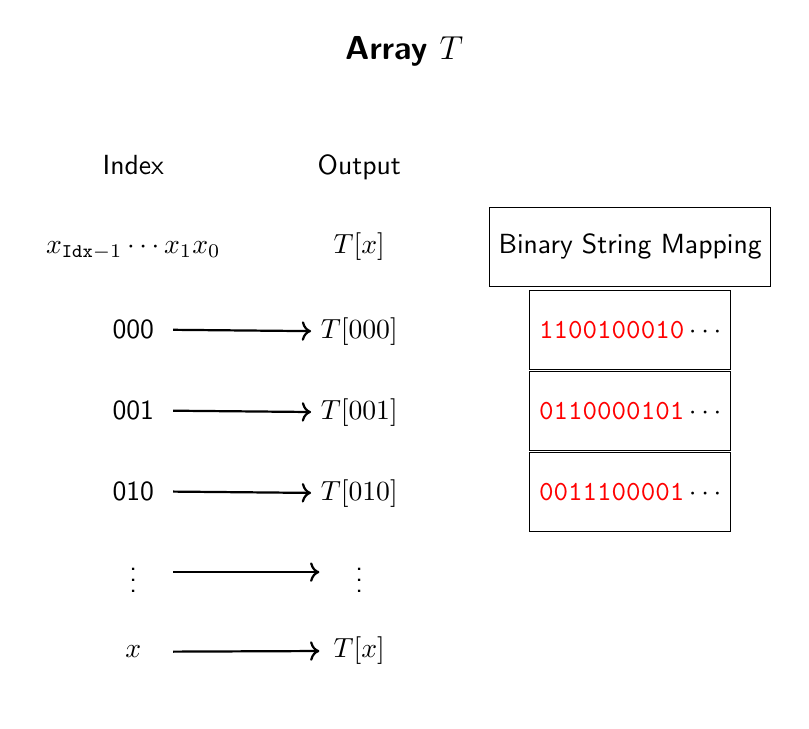
\begin{tikzpicture}
							% Define the number of bits for input and output
							\def\inputbits{3} % Example for in-bit
							\def\outputbits{2} % Example for out-bit
							\def\numofentries{8} % Number of entries in the array, 2^3 for the example
							
							% Draw the array table
							\matrix[matrix of nodes, nodes={draw, minimum size=10mm}, row sep=0pt, column sep=10mm, column 1/.style={nodes={draw=none}}, column 2/.style={nodes={draw=none}}] (array) {
								Index & Output & \\
								\(x_{\indexbit-1}\cdots x_1x_0\) & \(T[x]\) & Binary String Mapping \\
								000 & \(T[000]\) & \(\one\one\zero\zero\one\zero\zero\zero\one\zero\cdots\) \\
								001 & \(T[001]\) & \(\zero\one\one\zero\zero\zero\zero\one\zero\one\cdots\) \\
								010 & \(T[010]\) & \(\zero\zero\one\one\one\zero\zero\zero\zero\one\cdots\) \\
								\(\vdots\) & \(\vdots\) & \\
								$x$ & \(T[x]\) &\\
							};
							
							% Draw the function arrow and text
							\foreach \x in {3,...,7} {
								\draw[->, thick] (array-\x-1) -- (array-\x-2);
							}
							
							% Label for the Array
							\node[above=5mm of array] (label) {\large\bfseries Array \(T\)};
						\end{tikzpicture}
					\end{flushright}
				\end{minipage}
			\end{center}
			
			\begin{center}
				\begin{minipage}{.25\textwidth}\centering
					{\renewcommand{\arraystretch}{1.25}\begin{tabular}{|l|}
							\hline
							$k\gets\binaryfield^\lambda$\\
							\\
							\underline{\texttt{Lookup} ($x\in\binaryfield^{\indexbit}$):}\\
							\tab \textbf{return} $F(k,x)$\\
							\hline
					\end{tabular}}
				\end{minipage}
				\begin{minipage}{.7\textwidth}
					\begin{flushright}
						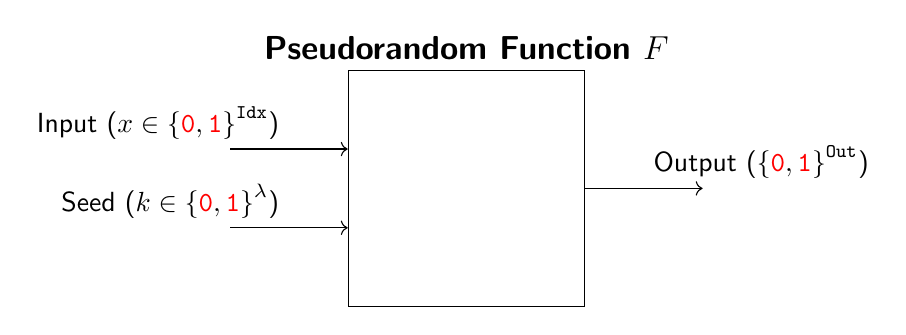
\begin{tikzpicture}
							% Define the number of bits for input and output
							\def\inputbits{in} % Replace 'in' with the actual number of input bits
							\def\outputbits{out} % Replace 'out' with the actual number of output bits
							
							% Draw the pseudorandom function F
							\node[draw, rectangle, minimum width=3cm, minimum height=3cm, label=above:{\large\bfseries Pseudorandom Function \( F \)}] (func) at (0,0) {};
							
							% Draw the input arrow and label
							\draw[->] (-3,0.5) -- node[above left] {Input (\(x\in\binaryfield^\indexbit\))} (func.west |- {0,0.5});
							
							% Draw the seed arrow and label
							\draw[->] (-3,-0.5) -- node[above left] {Seed ($k\in\binaryfield^\lambda$)} (func.west |- {0,-0.5});
							
							% Draw the output arrow and label
							\draw[->] (func.east) -- node[above right] {Output (\(\binaryfield^\outbit\))} (3,0);
							
						\end{tikzpicture}
					\end{flushright}
				\end{minipage}
			\end{center}
		\end{sectionbox}
		
		% Objectives
		\begin{sectionbox}
			\section*{Objectives}
			The primary aim of this research is to...
			\lipsum[1-3]
		\end{sectionbox}
		
		% References
		\begin{sectionbox}
			\section*{\textcolor{MainColor}{References}}
			[1] M. Rosulek, \textit{The Joy of Cryptography}, [Online]. Available: \url{https://joyofcryptography.com}\\
			\text{[2]} N. P. Smart, \textit{Cryptography Made Simple}. 1st ed. Springer International Publishing, 2016.\\
			\text{[3]} J. Katz and Y. Lindell, \textit{Introduction to Modern Cryptography}. 2nd ed. Chapman and Hall/CRC, 2014.
		\end{sectionbox}
		% End of the columns
	\end{multicols}
	
	% End of the document
\end{document}